\chapter{Implementazioni in LiSA}\label{chapter:lisa}



LiSA (\textbf{Li}brary for \textbf{S}tatic \textbf{A}nalysis) è un framework generico sviluppato come libreria open-source in Java che permette in modo facile, diretto e completo l'analisi statica tramite interpretazione astratta di semplici programmi multi linguaggio. Una basilare rappresentazione del flow dell'analisi in LiSA può essere vista in figura \ref{fig:lisaAnalysisFlow} e lo possiamo riassumere così: (1) un programma scritto in un linguaggio L viene passato al front-end appropriato che lo trascrive nel linguaggio intermedio compreso da LiSA basato su Control Flow Graph (generalmente un LiSA CFG per funzione), (2) LiSA poi analizza i CFGs creati con un algoritmo di ricerca del fix-point seguendo le linee guida passate da utente tramite la configurazione (ad esempio: domini da usare, parametri per l'algorito del fix-point, tipo di analisi interprocedurale), (3) infine LiSA esegue i semantics checks, anch'essi passati da utente, ed eventualmente genera warnings ed errori se l'analisi non ne rispetta i vincoli. 

LiSA mette a disposizione: (i) un linguaggio interno basato su control-flow graph estensibile e abbastanza generico da supportare i costrutti semantici di molti linguaggi di programmazione, (ii) una vasta gamma di front-end per la traduzione di programmi in LiSA CFGs, (iii) una base comune per lo sviluppo di nuovi domini astratti da usare nelle analisi (sia relazionali che non, più alcuni domini built-in) ed infine (iv) un algoritmo per il calcolo del fix-point dei LiSA CFGs con metodo di risoluzione basato su working-set list.

Durante la mia tesi ho lavorato soprattutto sulle componenti (iii) e (iv). Per prima cosa ho esteso l'algoritmo per il calcolo del fix-point affinchè fosse in grado di eseguire anche la fase discendente partendo da un post-fix-point precedentemente calcolato, ho aggiunto classi generiche come base per l'implementazione del dominio astratto degli insiemi non ridondanti di un altro dominio astratto (nonchè una implementazione concreta di ciò per gli intervalli) ed infine, per scopo sperimentale, una rudimentale versione del decoupling capace di usare domini diversi per salire e scendere nell'analisi.

\begin{figure}
    \centering
\usetikzlibrary{shadows}
\tikzset{every picture/.style={line width=0.75pt}} %set default line width to 0.75pt   
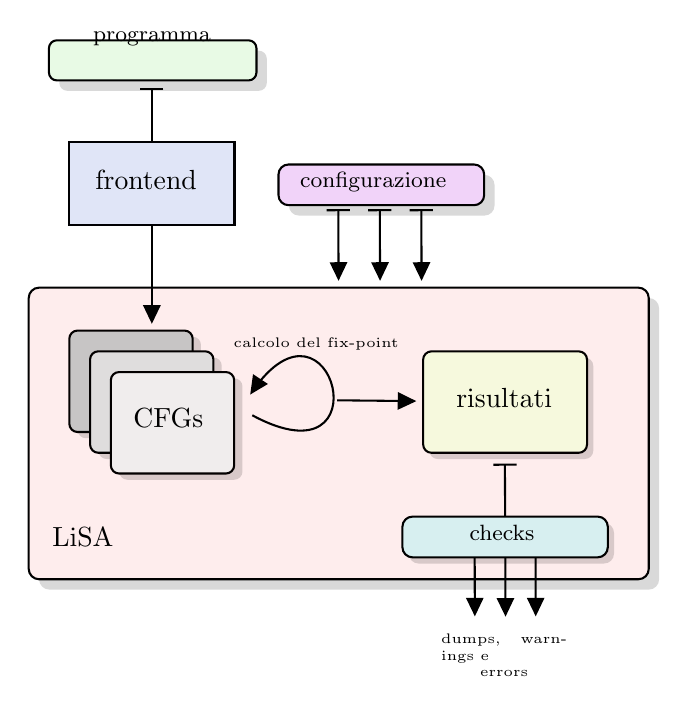
\begin{tikzpicture}[x=0.75pt,y=0.75pt,yscale=-1,xscale=1]
%uncomment if require: \path (0,336); %set diagram left start at 0, and has height of 336

%Shape: Rectangle [id:dp735576293814507] 
\draw  [color={rgb, 255:red, 0; green, 0; blue, 0 }  ,draw opacity=1 ][fill={rgb, 255:red, 254; green, 237; blue, 237 }  ,fill opacity=1 ][general shadow={fill={rgb, 255:red, 0; green, 0; blue, 0 }  ,shadow xshift=3.75pt,shadow yshift=-3.75pt, opacity=0.15 }] (10.44,145) .. controls (10.44,142.24) and (12.68,140) .. (15.44,140) -- (304.17,140) .. controls (306.93,140) and (309.17,142.24) .. (309.17,145) -- (309.17,275.5) .. controls (309.17,278.26) and (306.93,280.5) .. (304.17,280.5) -- (15.44,280.5) .. controls (12.68,280.5) and (10.44,278.26) .. (10.44,275.5) -- cycle ;
%Straight Lines [id:da23563586478588427] 
\draw    (69.77,44.13) -- (69.77,154.4) ;
\draw [shift={(69.77,157.4)}, rotate = 270] [fill={rgb, 255:red, 0; green, 0; blue, 0 }  ][line width=0.08]  [draw opacity=0] (8.93,-4.29) -- (0,0) -- (8.93,4.29) -- cycle    ;
\draw [shift={(69.77,44.13)}, rotate = 270] [color={rgb, 255:red, 0; green, 0; blue, 0 }  ][line width=0.75]    (0,5.59) -- (0,-5.59)   ;
%Shape: Rectangle [id:dp6301022803478207] 
\draw  [color={rgb, 255:red, 0; green, 0; blue, 3 }  ,draw opacity=1 ][fill={rgb, 255:red, 224; green, 229; blue, 247 }  ,fill opacity=1 ] (30,70) -- (109.57,70) -- (109.57,110) -- (30,110) -- cycle ;
%Rounded Rect [id:dp2844998293479686] 
\draw  [fill={rgb, 255:red, 232; green, 250; blue, 229 }  ,fill opacity=1 ][general shadow={fill={rgb, 255:red, 0; green, 0; blue, 0 }  ,shadow xshift=3.75pt,shadow yshift=-3.75pt, opacity=0.15 }] (20.17,24.7) .. controls (20.17,22.56) and (21.9,20.83) .. (24.03,20.83) -- (116.3,20.83) .. controls (118.44,20.83) and (120.17,22.56) .. (120.17,24.7) -- (120.17,36.3) .. controls (120.17,38.44) and (118.44,40.17) .. (116.3,40.17) -- (24.03,40.17) .. controls (21.9,40.17) and (20.17,38.44) .. (20.17,36.3) -- cycle ;
%Rounded Rect [id:dp015147798185889627] 
\draw  [fill={rgb, 255:red, 241; green, 211; blue, 249 }  ,fill opacity=1 ][general shadow={fill={rgb, 255:red, 0; green, 0; blue, 0 }  ,shadow xshift=3.75pt,shadow yshift=-3.75pt, opacity=0.15 }] (130.78,85.5) .. controls (130.78,82.83) and (132.94,80.67) .. (135.61,80.67) -- (225.03,80.67) .. controls (227.7,80.67) and (229.87,82.83) .. (229.87,85.5) -- (229.87,95.43) .. controls (229.87,98.1) and (227.7,100.27) .. (225.03,100.27) -- (135.61,100.27) .. controls (132.94,100.27) and (130.78,98.1) .. (130.78,95.43) -- cycle ;
%Shape: Rectangle [id:dp3167426310658905] 
\draw  [color={rgb, 255:red, 3; green, 0; blue, 0 }  ,draw opacity=1 ][fill={rgb, 255:red, 199; green, 197; blue, 197 }  ,fill opacity=1 ][general shadow={fill={rgb, 255:red, 0; green, 0; blue, 0 }  ,shadow xshift=3pt,shadow yshift=-2.25pt, opacity=0.15 }] (30,164.67) .. controls (30,162.46) and (31.79,160.67) .. (34,160.67) -- (85.44,160.67) .. controls (87.65,160.67) and (89.44,162.46) .. (89.44,164.67) -- (89.44,205.56) .. controls (89.44,207.76) and (87.65,209.56) .. (85.44,209.56) -- (34,209.56) .. controls (31.79,209.56) and (30,207.76) .. (30,205.56) -- cycle ;
%Shape: Rectangle [id:dp5390943849837029] 
\draw  [color={rgb, 255:red, 3; green, 0; blue, 0 }  ,draw opacity=1 ][fill={rgb, 255:red, 246; green, 249; blue, 221 }  ,fill opacity=1 ][general shadow={fill={rgb, 255:red, 0; green, 0; blue, 0 }  ,shadow xshift=2.25pt,shadow yshift=-2.25pt, opacity=0.15 }] (200.48,174.7) .. controls (200.48,172.49) and (202.27,170.7) .. (204.48,170.7) -- (275.44,170.7) .. controls (277.65,170.7) and (279.44,172.49) .. (279.44,174.7) -- (279.44,215.56) .. controls (279.44,217.76) and (277.65,219.56) .. (275.44,219.56) -- (204.48,219.56) .. controls (202.27,219.56) and (200.48,217.76) .. (200.48,215.56) -- cycle ;
%Shape: Rectangle [id:dp6482074079685427] 
\draw  [color={rgb, 255:red, 3; green, 0; blue, 0 }  ,draw opacity=1 ][fill={rgb, 255:red, 223; green, 221; blue, 221 }  ,fill opacity=1 ][general shadow={fill={rgb, 255:red, 0; green, 0; blue, 0 }  ,shadow xshift=3pt,shadow yshift=-2.25pt, opacity=0.15 }] (40,174.67) .. controls (40,172.46) and (41.79,170.67) .. (44,170.67) -- (95.44,170.67) .. controls (97.65,170.67) and (99.44,172.46) .. (99.44,174.67) -- (99.44,215.56) .. controls (99.44,217.76) and (97.65,219.56) .. (95.44,219.56) -- (44,219.56) .. controls (41.79,219.56) and (40,217.76) .. (40,215.56) -- cycle ;
%Shape: Rectangle [id:dp5665391899993595] 
\draw  [color={rgb, 255:red, 3; green, 0; blue, 0 }  ,draw opacity=1 ][fill={rgb, 255:red, 240; green, 237; blue, 237 }  ,fill opacity=1 ][general shadow={fill={rgb, 255:red, 0; green, 0; blue, 0 }  ,shadow xshift=3pt,shadow yshift=-2.25pt, opacity=0.15 }] (50,184.67) .. controls (50,182.46) and (51.79,180.67) .. (54,180.67) -- (105.44,180.67) .. controls (107.65,180.67) and (109.44,182.46) .. (109.44,184.67) -- (109.44,225.56) .. controls (109.44,227.76) and (107.65,229.56) .. (105.44,229.56) -- (54,229.56) .. controls (51.79,229.56) and (50,227.76) .. (50,225.56) -- cycle ;
%Straight Lines [id:da034591409315066324] 
\draw [line width=0.75]    (159.61,102.69) -- (159.71,133.69) ;
\draw [shift={(159.72,136.69)}, rotate = 269.81] [fill={rgb, 255:red, 0; green, 0; blue, 0 }  ][line width=0.08]  [draw opacity=0] (8.93,-4.29) -- (0,0) -- (8.93,4.29) -- cycle    ;
\draw [shift={(159.61,102.69)}, rotate = 269.81] [color={rgb, 255:red, 0; green, 0; blue, 0 }  ][line width=0.75]    (0,5.59) -- (0,-5.59)   ;
%Straight Lines [id:da8442899163237636] 
\draw [line width=0.75]    (179.61,102.69) -- (179.71,133.69) ;
\draw [shift={(179.72,136.69)}, rotate = 269.81] [fill={rgb, 255:red, 0; green, 0; blue, 0 }  ][line width=0.08]  [draw opacity=0] (8.93,-4.29) -- (0,0) -- (8.93,4.29) -- cycle    ;
\draw [shift={(179.61,102.69)}, rotate = 269.81] [color={rgb, 255:red, 0; green, 0; blue, 0 }  ][line width=0.75]    (0,5.59) -- (0,-5.59)   ;
%Straight Lines [id:da1808180600514191] 
\draw [line width=0.75]    (199.61,102.69) -- (199.71,133.69) ;
\draw [shift={(199.72,136.69)}, rotate = 269.81] [fill={rgb, 255:red, 0; green, 0; blue, 0 }  ][line width=0.08]  [draw opacity=0] (8.93,-4.29) -- (0,0) -- (8.93,4.29) -- cycle    ;
\draw [shift={(199.61,102.69)}, rotate = 269.81] [color={rgb, 255:red, 0; green, 0; blue, 0 }  ][line width=0.75]    (0,5.59) -- (0,-5.59)   ;
%Curve Lines [id:da7168976803847669] 
\draw    (118.17,201.5) .. controls (182.52,236.15) and (156.7,134.57) .. (118.33,189.78) ;
\draw [shift={(117.17,191.5)}, rotate = 303.47] [fill={rgb, 255:red, 0; green, 0; blue, 0 }  ][line width=0.08]  [draw opacity=0] (8.93,-4.29) -- (0,0) -- (8.93,4.29) -- cycle    ;
%Straight Lines [id:da3343995640969275] 
\draw [line width=0.75]    (159,194.28) -- (194.17,194.64) ;
\draw [shift={(197.17,194.67)}, rotate = 180.58] [fill={rgb, 255:red, 0; green, 0; blue, 0 }  ][line width=0.08]  [draw opacity=0] (8.93,-4.29) -- (0,0) -- (8.93,4.29) -- cycle    ;
%Straight Lines [id:da6598443106986112] 
\draw [line width=0.75]    (239.87,225.3) -- (240.16,295.5) ;
\draw [shift={(240.17,298.5)}, rotate = 269.76] [fill={rgb, 255:red, 0; green, 0; blue, 0 }  ][line width=0.08]  [draw opacity=0] (8.93,-4.29) -- (0,0) -- (8.93,4.29) -- cycle    ;
\draw [shift={(239.87,225.3)}, rotate = 269.76] [color={rgb, 255:red, 0; green, 0; blue, 0 }  ][line width=0.75]    (0,5.59) -- (0,-5.59)   ;
%Rounded Rect [id:dp7910872057944298] 
\draw  [fill={rgb, 255:red, 215; green, 239; blue, 240 }  ,fill opacity=1 ][general shadow={fill={rgb, 255:red, 0; green, 0; blue, 0 }  ,shadow xshift=2.25pt,shadow yshift=-2.25pt, opacity=0.15 }] (190.5,255.17) .. controls (190.5,252.5) and (192.66,250.33) .. (195.33,250.33) -- (284.61,250.33) .. controls (287.28,250.33) and (289.44,252.5) .. (289.44,255.17) -- (289.44,265.1) .. controls (289.44,267.77) and (287.28,269.93) .. (284.61,269.93) -- (195.33,269.93) .. controls (192.66,269.93) and (190.5,267.77) .. (190.5,265.1) -- cycle ;
%Straight Lines [id:da7891879484603097] 
\draw [line width=0.75]    (254.64,270.28) -- (254.71,295.36) ;
\draw [shift={(254.72,298.36)}, rotate = 269.83] [fill={rgb, 255:red, 0; green, 0; blue, 0 }  ][line width=0.08]  [draw opacity=0] (8.93,-4.29) -- (0,0) -- (8.93,4.29) -- cycle    ;
%Straight Lines [id:da9550393969063078] 
\draw [line width=0.75]    (225.31,270.28) -- (225.38,295.36) ;
\draw [shift={(225.39,298.36)}, rotate = 269.83] [fill={rgb, 255:red, 0; green, 0; blue, 0 }  ][line width=0.08]  [draw opacity=0] (8.93,-4.29) -- (0,0) -- (8.93,4.29) -- cycle    ;

% Text Node
\draw (59.33,197) node [anchor=north west][inner sep=0.75pt]   [align=left] {CFGs};
% Text Node
\draw (139.67,83) node [anchor=north west][inner sep=0.75pt]   [align=left] {{\footnotesize configurazione}};
% Text Node
\draw (38.67,15.25) node [anchor=north west][inner sep=0.75pt]  [font=\footnotesize] [align=left] {\begin{minipage}[lt]{44.44pt}\setlength\topsep{0pt}
\begin{center}
programma
\end{center}

\end{minipage}};
% Text Node
\draw (41,82) node [anchor=north west][inner sep=0.75pt]   [align=left] {frontend};
% Text Node
\draw (20.33,254) node [anchor=north west][inner sep=0.75pt]   [align=left] {LiSA};
% Text Node
\draw (107.67,162.75) node [anchor=north west][inner sep=0.75pt]  [font=\tiny] [align=left] {calcolo del fix-point};
% Text Node
\draw (215,187) node [anchor=north west][inner sep=0.75pt]   [align=left] {risultati};
% Text Node
\draw (221.33,253.08) node [anchor=north west][inner sep=0.75pt]   [align=left] {{\footnotesize checks}};
% Text Node
\draw (207.67,305.42) node [anchor=north west][inner sep=0.75pt]  [font=\tiny] [align=left] {\begin{minipage}[lt]{45.52pt}\setlength\topsep{0pt}
dumps, warnings e
\begin{center}
errors
\end{center}

\end{minipage}};


\end{tikzpicture}
    \caption{Schema del flow dell'analisi in LiSA}
    \label{fig:lisaAnalysisFlow}
\end{figure}

\section{LiSA}
In questa sezione faremo una overview della archutettura di LiSA focalizzandoci sulla struttura della rappresentazione interna dei programmi, sulle interfacce attraverso cui è possibile definire nuovi domini astratti e sull'organizzazione della vera e propria analisi statica (andando a guardarne le componenti e gli algoritmi).

\subsection{I CFG di LiSA}
La struttura dei CFG in LiSA è progettata per essere il più flessibile possibile così da essere in grado di rappresentare il maggior numero di costrutti semantici provenienti da più linguaggi di programmazione. Un LiSA CFG ha gli \texttt{Statement} come nodi (ognuno con il proprio significato semantico) e gli \texttt{Edge} come archi (i quali modellano il flusso di dati durante l'esecuzione del programma). 

\subsubsection{\texttt{Statement}}
Uno \texttt{Statement} rappresenta un costrutto semantico base di un linguaggio di programmazione che non modifica il flusso di esecuzione. Uno \texttt{Statement} che lascia un valore sullo stack è detto \texttt{Expression}, che è una sotto classe di \texttt{Statement}. La maggior parte delle \texttt{Expression} rappresentano operazioni base comuni a molti linguaggio (come addizione, sottrazione, e tutte le altre operazioni aritmetiche, operazioni sulle stringhe come concatenazione o lunghezza, operazioni logiche su booleani come and e or e così via). Una sotto-classe particolare di \texttt{Expression} è \texttt{Call}. Esistono molti tipi di \texttt{Call} in LiSA, ma riassuntivamente queste rappresentano chiamate ad altre funzioni, quindi altri CFG. Le \texttt{Call} vengono gestite tramite una classe che implementa l'interfaccia \texttt{InterproceduralAnalysis}, il compito di una di queste classi è proprio di gestire l'interproceduralità di un programma, ovvero la possibilità di avere, in una funzione, chiamate ad altre funzioni (o a se stesse, quindi chiamate ricorsive). In figura \ref{fig:gerarchiaStatement} si può vedere una sommaria e non completa gerarchia della classe \texttt{Statement}.

\begin{figure}[ht]
	\centering
	\includegraphics[width=0.9\textwidth]{Immagini/gerarchiaStatement.png}
	\caption{Gerarchia della classe \texttt{statement}}
	\label{fig:gerarchiaStatement}
\end{figure}

\subsubsection{\texttt{Edge}}
La classe \texttt{Edge} collega tra di loro due nodi. Esistono tre tipi di \texttt{Edge}: \texttt{SequentialEdge}, modella un flusso senza condizione e sequenziale dal nodo di origine al nodo target, \texttt{TrueEdge}, modella un flusso condizionale se la condizione nel nodo di origine è vera, \texttt{FalseEdge}, modella un flusso condizionale se la condizione nel nodo di origine è falsa.
\\

\texttt{Edge} e \texttt{Statement} modificano le istanze del dominio astratto attraverso, rispettivamente, i metodi \texttt{traverse}, che agisce sul post-state del nodo di origine e consegna il valore trasformato al pre-state del nodo target, e \texttt{semantics}, che trasforma il pre-state di un nodo nel suo post-state. Più precisamente però non è la classe \texttt{Statement} che modifica il dominio astratto, infatti ogni \texttt{Statement} viene trascritto in una composizione di \texttt{SymbolicExpression} a run-time durante l'analisi. Ogni \texttt{SymbolicExpression} ha un significato semantico ben preciso e le istanze del dominio astratto definiscono gli effetti semantici su quest'ultime e non sugli \texttt{Statement}. Possiamo vedere gli \texttt{Statement} come la sintassi e le \texttt{SymbolicExpression} come la semantica dei CFG in LiSA. Le \texttt{SymbolicExpression} si dividono in due principali tipi di espressione, abbiamo le \texttt{HeapExpression}, ovvero le espressioni che modellano le operazioni sul'heap (come \texttt{HeapAllocation}, \texttt{AccessChild}), e le \texttt{ValueExpression}, che modellano modifiche e operazione sul valore di variabili e costanti (qui per esempio abbiamo \texttt{Addition}, \texttt{LessOrEqual}, \texttt{And}, \texttt{Modulo}, etc..). In figura \ref{fig:gerarchiaSymbolic} qua sotto si vede la non completa gerarchia delle \texttt{SymbolicExpression}.

\begin{figure}[ht]
	\centering
	\includegraphics[width=0.9\textwidth]{Immagini/gerarchiaSymbolicExpression.png}
	\caption{Gerarchia della classe \texttt{statement}}
	\label{fig:gerarchiaSymbolic}
\end{figure}


Per fare un esempio prendiamo in considerazione lo statement \texttt{x = a + b} in un linguaggio non tipato (come Python), in cui non sappiamo i tipi dei valori di \texttt{a} e \texttt{b}. Questo statement in LiSA può essere tradotto in due espressioni simboliche, una per le parte sinistra, ovvero un riferimento alla variabile \texttt{x}, che può essere ulteriormente processata dal dominio astratto che modula l'heap, e una per la parte destra e modella la semantica dell'addizione \texttt{a + b}. Questa può anche controllare i tipi delle due variabili di \texttt{a} e \texttt{b} a run-time e in alcuni casi generare una \texttt{SymbolicExpression} che rappresenta l'addizione tra interi (se le due variabili possono avere valori numerici interi) e in altri casi una che rappresenta la concatenazione di stringhe (se entrambe possono contenere stringhe), o qualsiasi altro tipo di operazione modellata tramite il \texttt{+} che dipende dalle caratteristiche dei suoi operandi.
Questa traduzione run-time degli \texttt{Statement} in più \texttt{SymbolicExpression} rende i CFG di LiSA dinamici e plastici, quindi capaci di rappresentare un grande numero di costrutti semantici e la possibilità di modellare le funzioni della maggior parte dei linguaggi. Il compito del front-end in LiSA sarà quello di trasformare un programma scritto in un qualsiasi linguaggio di programmazione in un insieme di CFG comprendibili a LiSA, fatti di \texttt{Statement} (anche language-specific) e \texttt{edge}, e capaci di simulare \textit{completamente} la semantica del programma originale.

\subsection{Domini astratti in LiSA}\label{sec:abstractDomainLiSA}
Ora parleremo invece di come sono definiti in LiSA i domini astratti. Ogni dominio in LiSA implementa due interfacce: \texttt{SemanticDomain}, che rende il dominio capace di valutare l'esecuzione di \texttt{SymbolicExpression} su istanze di esso, e \texttt{Lattice}, che fornisce al dominio le caratteristiche di un reticolo. Ora vediamo queste due interfacce più nel dettaglio.

\subsubsection{\texttt{SemanticDomain}}\label{subsec:semanticDomain}
L'interfaccia \texttt{SemanticDomain} è parametrica all'istanza concreta D, agli \texttt{Identifier} I e alle \texttt{SymbolicExpression} E. Rappresenta un dominio che è capace di ragionare sulla semantica delle \texttt{SymbolicExpression} di tipo E su \texttt{Identifier} di tipo I. Un dominio semantico D deve implementare i seguenti metodi:
\begin{itemize}
\setlength\itemsep{0.1em}
    \item \texttt{D assign(I id, E exp)}: restituisce un istanza del dominio in cui viene assegnato il valore di \texttt{exp} ad \texttt{id};
    \item \texttt{D assume(E exp)}: restituisce una istanza del dominio in cui si assume che \texttt{exp} sia vera;
    \item \texttt{D forgetIdentifier(I id)}: restituisce una istanza del dominio in cui viene scordata qualsiasi informazione riguardante l'identificatore \texttt{id};
    \item \texttt{D forgetIdentifiers(Collection<I> ids)}: restituisce una istanza del dominio in cui viene scordata qualsiasi informazione riguardante gli identificatori \texttt{ids};
    \item \texttt{Satisfiability satisfies(E exp)}: resituisce un valore (tra \texttt{SATISFIED}, \texttt{UNKNOWN}, \texttt{NOT\_SATISFIED} e \texttt{BOTTOM}) che indica se la espressione \texttt{exp} è soddisfatta nel dominio corrente;
    \item \texttt{D smallStepSemantics(E exp)}: resitutisce una istanza del dominio modificata dagli effetti della espressione \texttt{exp};
\end{itemize}

\subsubsection{\texttt{Lattice}}\label{subsec:lattice}
L'interfaccia \texttt{Lattice} è parametrica all'istanza concreta L. Un reticolo in LiSA deve implementare questi metodi:
\begin{itemize}
\setlength\itemsep{0.1em}
    \item \texttt{boolean lessOrEqual(L other)}: questo metodo definisce l'ordine parziale del reticolo e restituisce \texttt{true} se l'oggetto su cui viene chiamato è in relazione con \texttt{other};
    \item \texttt{L lub(L other)}: definisce l'operazione di least upper bound e restituisce il lub tra questo oggetto e \texttt{other};
    \item \texttt{L glb(L other)}: definisce l'operazione di greatest lower bound e restituisce il glb tra questo oggetto e \texttt{other};
    \item \texttt{L top(L other)}: restituisce l'elemento \(\top\) del reticolo;
    \item \texttt{L bottom(L other)}: restituisce l'elemento \(\perp\) del reticolo;
    \item \texttt{L widening(L other)}: definisce l'operazione di widening del reticolo e restituisce il widening tra questo oggetto e \texttt{other};
    \item \texttt{L narrowing(L other)}: definisce l'operazione di narrowing del reticolo e restituisce il narrowing tra questo oggetto e \texttt{other} (di defualt il narrowing esegue il glb);
    \item \texttt{boolean isTop()}: restiuisce \texttt{true} se l'istanza su cui viene chiamata è l'elemento \(\top\);
    \item \texttt{boolean isBottom()}: restiuisce \texttt{true} se l'istanza su cui viene chiamata è l'elemento \(\perp\);
\end{itemize}
In LiSA sono definite alcune implementazioni base di reticoli con comportamenti simili. Innanzitutto è definita l'interfaccia \texttt{BaseLattice} che estende \texttt{Lattice}, la quale definisce i casi base comuni a tutti i reticoli (ovvero le relazioni tra gli oggetti e gli elementi \(\top\) e \(\perp\)). A partire da questa sono poi implementate le classi astratte che definiscono il \texttt{SetLattice<E>} e \texttt{InverseSetLattice<E>} visti nell'esempio \ref{ex:setLattice} e il \texttt{FunctionalLattice<K,E>}, parametrico al tipo K del dominio della funzione e al tipo E del codominio nonchè dominio di un reticolo, visto nell'esempio \ref{ex:functionalLattice}. 


\subsubsection{Lo stato dell'analisi in LiSA: \texttt{AnalysisState}}

Vediamo ora come LiSA organizza lo stato dell'analisi. Lo stato dell'analisi è l'oggetto che viene mappato ad ogni nodo del CFG e indica l'astrazione della semantica  concreta che si vuole approssimare in quel punto di programma (solitamente in LiSA è una astrazione della collecting semantics, ovvero la semantica che ci dice tutti i possibili valori della memoria in un dato punto di programma o equivalentemente l'insieme di tutti gli stati attraversabili durante l'esecuzione del programma). Lo stato dell'analisi è costruito modularmente bottom-up come mostrato in figura \ref{fig:analysisState}.

\begin{figure}
\centering
\tikzset{every picture/.style={line width=0.75pt}} %set default line width to 0.75pt  
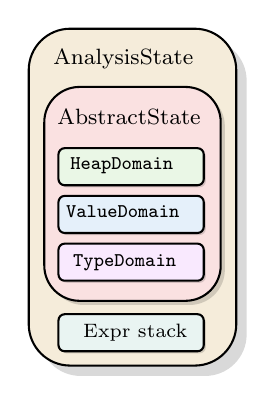
\begin{tikzpicture}[x=0.75pt,y=0.75pt,yscale=-1,xscale=1]
%uncomment if require: \path (0,300); %set diagram left start at 0, and has height of 300

%Rounded Rect [id:dp5259274252543102] 
\draw  [fill={rgb, 255:red, 245; green, 236; blue, 218 }  ,fill opacity=1 ][general shadow={fill={rgb, 255:red, 0; green, 0; blue, 0 }  ,shadow xshift=3.75pt,shadow yshift=-3.75pt, opacity=0.15 }] (20.67,194.89) .. controls (20.67,205.94) and (29.62,214.89) .. (40.67,214.89) -- (100.67,214.89) .. controls (111.71,214.89) and (120.67,205.94) .. (120.67,194.89) -- (120.67,72.59) .. controls (120.67,61.55) and (111.71,52.59) .. (100.67,52.59) -- (40.67,52.59) .. controls (29.62,52.59) and (20.67,61.55) .. (20.67,72.59) -- cycle ;
%Rounded Rect [id:dp40217338693406735] 
\draw  [fill={rgb, 255:red, 250; green, 225; blue, 225 }  ,fill opacity=1 ][general shadow={fill={rgb, 255:red, 0; green, 0; blue, 0 }  ,shadow xshift=1.5pt,shadow yshift=-1.5pt, opacity=0.15 }] (28.17,166.69) .. controls (28.17,176.08) and (35.78,183.69) .. (45.17,183.69) -- (96.17,183.69) .. controls (105.56,183.69) and (113.17,176.08) .. (113.17,166.69) -- (113.17,97.64) .. controls (113.17,88.25) and (105.56,80.64) .. (96.17,80.64) -- (45.17,80.64) .. controls (35.78,80.64) and (28.17,88.25) .. (28.17,97.64) -- cycle ;
%Shape: Rectangle [id:dp7147766556498871] 
\draw  [fill={rgb, 255:red, 249; green, 233; blue, 254 }  ,fill opacity=1 ][general shadow={fill={rgb, 255:red, 0; green, 0; blue, 0 }  ,shadow xshift=0.75pt,shadow yshift=-0.75pt, opacity=0.15 }] (35,159.14) .. controls (35,157.49) and (36.34,156.14) .. (38,156.14) -- (102,156.14) .. controls (103.66,156.14) and (105,157.49) .. (105,159.14) -- (105,171) .. controls (105,172.66) and (103.66,174) .. (102,174) -- (38,174) .. controls (36.34,174) and (35,172.66) .. (35,171) -- cycle ;
%Shape: Rectangle [id:dp6945641114766774] 
\draw  [color={rgb, 255:red, 0; green, 0; blue, 0 }  ,draw opacity=1 ][fill={rgb, 255:red, 229; green, 240; blue, 250 }  ,fill opacity=1 ][general shadow={fill={rgb, 255:red, 0; green, 0; blue, 0 }  ,shadow xshift=0.75pt,shadow yshift=-0.75pt, opacity=0.15 }] (35,136.14) .. controls (35,134.49) and (36.34,133.14) .. (38,133.14) -- (102,133.14) .. controls (103.66,133.14) and (105,134.49) .. (105,136.14) -- (105,148) .. controls (105,149.66) and (103.66,151) .. (102,151) -- (38,151) .. controls (36.34,151) and (35,149.66) .. (35,148) -- cycle ;
%Shape: Rectangle [id:dp6352913495307582] 
\draw  [fill={rgb, 255:red, 234; green, 247; blue, 230 }  ,fill opacity=1 ][general shadow={fill={rgb, 255:red, 0; green, 0; blue, 0 }  ,shadow xshift=0.75pt,shadow yshift=-0.75pt, opacity=0.15 }] (35,113.14) .. controls (35,111.49) and (36.34,110.14) .. (38,110.14) -- (102,110.14) .. controls (103.66,110.14) and (105,111.49) .. (105,113.14) -- (105,125) .. controls (105,126.66) and (103.66,128) .. (102,128) -- (38,128) .. controls (36.34,128) and (35,126.66) .. (35,125) -- cycle ;
%Shape: Rectangle [id:dp47123715282050216] 
\draw  [fill={rgb, 255:red, 233; green, 244; blue, 242 }  ,fill opacity=1 ][general shadow={fill={rgb, 255:red, 0; green, 0; blue, 0 }  ,shadow xshift=0.75pt,shadow yshift=-0.75pt, opacity=0.15 }] (35,193.14) .. controls (35,191.49) and (36.34,190.14) .. (38,190.14) -- (102,190.14) .. controls (103.66,190.14) and (105,191.49) .. (105,193.14) -- (105,205) .. controls (105,206.66) and (103.66,208) .. (102,208) -- (38,208) .. controls (36.34,208) and (35,206.66) .. (35,205) -- cycle ;


% Text Node
\draw (31,61) node [anchor=north west][inner sep=0.75pt]  [font=\footnotesize] [align=left] {AnalysisState};
% Text Node
\draw (33,90) node [anchor=north west][inner sep=0.75pt]  [font=\footnotesize] [align=left] {AbstractState};
% Text Node
\draw (39.2,113.2) node [anchor=north west][inner sep=0.75pt]   [align=left] {{\scriptsize \texttt{HeapDomain}}};
% Text Node
\draw (37.2,136.2) node [anchor=north west][inner sep=0.75pt]   [align=left] {{\scriptsize \texttt{ValueDomain}}};
% Text Node
\draw (40.6,159.8) node [anchor=north west][inner sep=0.75pt]   [align=left] {{\scriptsize \texttt{TypeDomain}}};
% Text Node
\draw (45.4,193.4) node [anchor=north west][inner sep=0.75pt]   [align=left] {{\scriptsize Expr stack}};
\end{tikzpicture}
    \caption{Architettura dello stato dell'analisi in LiSA}
    \label{fig:analysisState}
\end{figure}

La classe che definisce lo stato dell'analisi è \texttt{AnalysisState}. \'E formato da due componenti: un \texttt{AbstractState} e lo stack delle espressioni, ovvero l'insieme di \texttt{SymbolicExpression} che rimangono sullo stack dopo il calcolo di una espressione (è importante notare che questa è solo una visione sommaria dell'\texttt{AnalysisState}). Il principale compito di questa classe è quello però di fare da wrap tra l'\texttt{AbstractState} e informazioni semantiche aggiuntive utili al raggiungimento del fix-point durante il calcolo dell'analisi. L'\texttt{AnalysisState} implementa entrambe le interfacce mostrate prima (\hyperref[subsec:lattice]{\texttt{Lattice}} e \hyperref[subsec:semanticDomain]{\texttt{SemanticDomain}}) rendendolo un oggetto sia capace di ragionare sulla semantica delle espressioni simboliche che un sistema ordinato con le caratteristiche di un reticolo. Ogni sua componente, scendendo gerarchicamente nella struttura, implementa queste due interfacce. L'\texttt{AbstractState} è l'astrazione dello stato della memoria e, come si vede dall'immagine, è composto da tre sotto-domini (ognuno dei quali implementa le interfacce \hyperref[subsec:lattice]{\texttt{Lattice}} e \hyperref[subsec:semanticDomain]{\texttt{SemanticDomain}}): 
\begin{itemize}
\setlength\itemsep{0.1em}
    \item un \texttt{HeapDomain} che è responsabile di tracciare l'evoluzione dello stato della memoria dinamica durante l'esecuzione. Opera prima del \texttt{ValueDomain} e risolve gli indirizzi traducendo le espressioni simboliche e rinominando le variabili in modo tale che il \texttt{ValueDomain} possa comprenderle e si preocccupi \textit{solamente} di tracciarne le proprietà;
    
    \item un \texttt{ValueDomain} che è responsabile di tracciare proprietà astratte (come per esempio il valore astratto) delle variabili (possibilmente pre-processate e riscritte prima dall'\texttt{HeapDomain}) del programma. In LiSA è possibile definire \texttt{ValueDomain} sia relazionali (come i Polyhedra) sia non. Per quest'ultimi è definito dentro LiSA una classe base chiamata \texttt{Environment} che estende  \texttt{FunctionalLattice<Identifier, L>} ed implementa \texttt{SemanticDomain}, ed è capace di tracciare un valore del dominio astratto \texttt{L} (che può essere per esempio un Interval, un Sign, un Modulo) ad ogni identificatore tenuto in memoria. Va sottolineato che il dominio \texttt{L} di un \texttt{Environment} ha si la struttura reticolare, ed estende \texttt{Lattice}, e può anche ragionare semanticamente sulle \texttt{SymbolicExpression} senza però implementare \texttt{SemanticDomain}. Infatti per il caso specifico dei domini non-relazionali gestiti tramite \texttt{Environment} il dominio astratto si costruirà attraverso l'interfaccia \texttt{NonRelationalDomain} che ha solo un sottoinsieme dei metodi di \texttt{SemanticDomain}. Per capire perchè pensiamo ai metodi \texttt{assign}, \texttt{forgetIdentifier/s} in \texttt{SemanticDomain}. La definizione di questi metodi, potenzialmente, è uguale per tutti i dominio non-relazionali, ed infatti di queste se ne prende carico la classe \texttt{Environment}, lasciando alla creazione dei domini astratti non-relazionali solo la necessità di definire: (i) le operazioni riguardanti la struttura reticolare del dominio (lub, glb, lessOrEqual, \(\cdots\)), e (ii) la logica per la valutazione delle espressioni simboliche;
    
    \item un \texttt{TypeDomain} che è un \texttt{ValueDomain} che associa ad ogni variabile l'insieme dei possibili tipi a run-time delle variabili. Questa può essere usata durante l'analisi per generare espressioni simboliche specifiche a seconda dei tipi delle variabili coinvolte nello statement;
\end{itemize}

L'\texttt{AbstractState} principlamente fa quindi da coordinatore tra l'\texttt{HeapDomain} e il \texttt{ValueDoamin}, passando all'ultimo le espressioni tradotte e gli identificatori trasformati dal primo quando i due mondi devono comunicare e invece compartizzando e separando i due domini quando le espressioni riguardano solo su uno dei due.

\subsection{Calcolo del fix-point in LiSA}\label{sec:fix-pointLiSA}
Abbiamo visto nel capitolo [??] che fare interpretazione astratta (sezione [??]) non significa altro che trovare una soluzione ad un sistema di equazioni costruito a partire dal CFG del programma. Tutte le soluzioni del sistema sono per definizione suoi fix-point e quindi cercare la soluzione significa cercarne un fix-point (possibilmente il più preciso, ovvero il least fix-point). Come viene mostrato nell'articolo di Cousot [??] qualsiasi metodo caotico di risoluzione ci permette di ottenere una soluzione del sistema (non necessariamente la minima). Tra tutti questi metodi ci conviene usarne uno efficiente e che sfrutti la struttura del CFG in modo da velocizzare la convergenza verso un fix-point. L'algoritmo che viene utilizzato in LiSA per la risoluzione del sistema di equazioni è quello classico basato su working-set e prima delle mie modifiche seguiva la definizione in pseudo-codice fornita in \ref{alg:fixpointAsc}.

\begin{algorithm}
	\caption{Algoritmo per il calcolo del fix-point con working-set list con solo fase ascendente}
	\label{alg:fixpointAsc}
	\begin{algorithmic}[1]
		\Statex
		%\Function{MST-Prim}{grafo G, funzione\_peso $\omega$, nodo\_radice r}\\
        
		\Let{\textit{result}}{\{\}}
        \Let{\textit{ws}}{\(\{st_0\}\)}
        \While{\(ws\neq \emptyset\)}
            \Let{\textit{st}}{\(pop(ws)\)}
            \Let{\(in_{st}\)}{\(\bigsqcup\{traverse_{prev\rightarrow st}(out_{prev})\ |\ prev \in preds(st)\}\)}
            \Let{\(out_{st}\)}{\(semantics_{st}(in_{st})\)}
            \If{\textbf{not }\(out_{st} \leq result[st]\)}
                \If{il widening threshold è stato raggiunto}
                    \Let{\(result[st]\)}{\(result[st]\nabla out_{st}\)}
                \Else
                    \Let{\(result[st]\)}{\(result[st]\sqcup out_{st}\)}
                \EndIf
                \Let{\(ws\)}{\(ws\cup succs(st)\)}
            \EndIf
        \EndWhile
		\State \Return{\textit{result}}
        
		%\EndFunction
	\end{algorithmic}
\end{algorithm}

Nell'algoritmo \(result\) è una mappa che associa ogni statement del grafo ad uno stato astratto (in LiSA in sostanza è una istanza di \texttt{Map<Statement, AnalysisState>}). All'inizio la mappa è vuota (che può essere visto come il partire dall'elemento \(\perp\)). \(ws\) è la lista contente gli statement ancora da calcolare e inizialmente viene caricata con l'entry-point del CFG (ovvero \(st_0\)). Si entra poi in un ciclo while che viene ripetuto finchè nella \(ws\) sono presenti statement. I passaggi all'interno del while sono:
\begin{enumerate}
\itemsep0em 
    \item si estrae un elemento dal \(ws\);
    \item viene calcolato il pre-state dello statement facendo il lub tra tutti i post-state degli statement precedenti al corrente, applicando ad essi la funzione semantica propria dell'arco che connette i due nodi (in LiSA questa sarebbe il metodo \texttt{traverse} delle istanze della classe \texttt{Edge});
    \item si calcola il post-state dello statement facendo passare il pre-state attraverso la funzione semantica propria del nodo corrente (in LiSA questa è il metodo \texttt{semantics} delle istanze della classe \texttt{Statement}).
    \item si controlla se il post-state del nodo sia minore o uguale allo stato astratto mappato a quello statement in \(result\). Se ciò che abbiamo calcolato nel post-state è minore od uguale a quello che abbiamo già possiamo evitare di aggiungere i nodi successivi al corrente in \(ws\), perchè siamo sicuri di non poter dare loro nessuna informazione in più che già non gli abbiamo dato precedentemente e che quindi non li aiuterebbe a cambiare il loro post-state. Se invece non è minore o uguale bisogna aggiornare \(result\) e propagare il cambiamento a tutti gli statement successivi a quello corrente sotto analisi. 
    \item se siamo entrati nel corpo dell'if a riga 7 vuol dire che dobbiamo aggiornare \(result\). Come abbiamo visto nel capitolo sull'intepretazione astatta per raggiungere un fix-point (che sia il least fix-point o una approssimazione di esso) dobbiamo applicare un'operazione di join tra i risultati degli step della iterazione sul sistema di equazioni. Questa operazione di join deve essere un operatore di upper bound (quindi il lub o una sua approssimazione, per esempio il widening). Per scegliere se usare il widening o il lub settiamo a priori nell'analisi un valore di threshold. Una volta passati threshold volte per uno statement durante l'analisi passiamo dall'usare il lub all'usare il widening. Questa logica decisionale ci permette di garantire la finitudine dell'analisi, infatti siamo sicuri che dopo un numero finito di step si cominci ad usare il widening, il quale a sua volta, come abbiamo visto, ci garantisce la convergenza. Infine, dopo aver aggiornato \(result\), dobbiamo garantire di propagare i cambiamenti effettuati e quindi inseriamo tutti gli statement successivi al corrente nel \(ws\). 
\end{enumerate}
Prima o poi non ci sono più aggiornamenti da fare a \(result\) e quindi non vengono più aggiunti statement a \(ws\), che di conseguenza si svuota e rende falsa la condizione del ciclo while alla riga 3 terminando la computazione e lasciando in \(result\) un fix-point, e quindi una soluzione, del sistema di equazioni generato a partire dal CFG.
\\

\definecolor{keywordsColor}{rgb}{0.5, 0.0, 0.333}
\lstset
    {
    basicstyle=\footnotesize\ttfamily,
    breaklines=true,
    keywordstyle=\color{keywordsColor}\bfseries,
    language=Java, 
    numbers=none,
    %showspaces=true,
    literate={\ \ }{{\ }}1,
    frame=single,
    breaklines=true
    }

\subsection{Come fare una semplice analisi in LiSA}
In questa piccola sezione vedremo come utilizzare effettivamente LiSA. Il frammento di codice qui di seguito ci permette di analizzare il programma presente in \texttt{programFilePath} utilizzando il \texttt{Frontend} appropriato per il linguaggio in cui è scritto. 
\label{code:simpleAnalysisAsc}
\begin{lstlisting}[belowskip=-1.1 \baselineskip]
LiSAConfiguration conf = new LiSAConfiguration();
conf.abstractState = LiSAFactory.getDefaultFor(
				AbstractState.class, 
				getDefaultFor(HeapDomain.class), 
				new Interval(),
				new TypeEnvironment<>(new InferredTypes()));
conf.wideningThreshold = 5;
conf.analysisGraphs = GraphType.DOT;
conf.workdir = outputDirectory;
Program program = Frontend.processFile(programFilePath);
LiSA lisa = new LiSA(configuration);
lisa.run(program);
\end{lstlisting}
Bisogna inanzitutto configurare l'analisi attraverso un oggetto della classe \texttt{LiSAConfiguration}. Un parametro obbligatorio è lo stato astratto da utilizzare e le sue componenti. In questo caso viene utilizzato quello di default per l'\texttt{HeapDomain}, il dominio non-relazionale \texttt{Interval}, che verrà wrappato in un \texttt{ValueEnvironment}, per il \texttt{ValueDomain} e il dominio con tipi dedotti per il \texttt{TypeDomain}. Viene poi settato il tipo di output con cui vogliamo visualizzare i risultati e la cartella in cui vogliamo che venga messo l'output generato dall'analisi. Viene generato il programma (che semplificando può essere visto come iuna collezione di CFG) tramite il \texttt{Frontend}. Infine viene lanciata l'analisi tramite un oggetto   della classe \texttt{LiSA} passando configurazioni e programma da analizzare. In figura \ref{fig:risultatoDOTAsc} è mostrato l'output generato in DOT con queste configurazioni per il programma mostrato in \ref{fig:codiceEsempio2}.
\begin{figure}[ht]
	\centering
	\includegraphics[width=0.8\textwidth]{Immagini/graphviz.png}
	\caption{Risultato in formato DOT dell'analisi con solo fase ascendente del codice in \ref{fig:codiceEsempio2}}
	\label{fig:risultatoDOTAsc}
\end{figure}
\\

Fino'ora abbiamo introdotto tutte le nozioni matematiche e teoriche necessarie per capire come funzioni l'analisi statica tramite interpretazione astratta (nel capitolo []) ed abbiamo visto come questi concetti vengono applicati all'interno di LiSA (nella sezione [] di questo capitolo). Da questo punto in poi verrà spiegato il contributo che io ho dato per espandere la libreria, guardando nel dettaglio ogni implementazione. 

\section{Dominio dell'insieme delle parti finite e non ridondanti in LiSA}

Come abbiamo detto nella piccola introduzione al concetto di \texttt{ValueDomain} in LiSA è possibile sviluppare domini sia relazionali che non. Lo sviluppo nei due casi prende "percorsi" diversi, e questo perchè, abbiamo detto, molte operazioni sono comuni a tutti i domini non-relazionali e quindi aveva senso avere un strato in più che si prendesse carico di queste operazioni comuni, ovvero l'\texttt{Environment}, semplificando per l'utente l'operazione di sviluppare domini non-relazionali. Per questo motivo l'introduzione di un sistema generico per lo sviluppo del dominio dell'insieme delle parti finite e non ridondanti di un altro dominio astratto, già definito in LiSA, ha dovuto coprire entrambi casi. Partiamo dal caso generale. 

\subsection{Il caso generale}

Nella sezione \ref{sec:abstractDomainLiSA} abbiamo mostrato le caratteristiche che deve avere un dominio astratto in LiSA (sottoforma delle interfacce che deve implementare). In \ref{code:nonRedundantPowerset} è mostrata la definizione (non completa) della classe che implementa la versione più generale del concetto di dominio dei sottinsiemi finiti e non ridondanti di un altro dominio.
%(a partire dalla quale si possono sviluppare sia domini relazionali che non).
\begin{algorithm}
\lstset{frame=none}
\begin{lstlisting}[belowskip=-1.1 \baselineskip]
public abstract class NonRedundantPowerset<
        C extends NonRedundantPowerset<C, T, E, I>,
        T extends SemanticDomain<T, E, I> & Lattice<T>,
        E extends SymbolicExpression,
        I extends Identifier> 
    extends SetLattice<C, T> 
    implements SemanticDomain<C, E, I> {

    public final T valueDomain;
    
    public NonRedundantPowerset(Set<T> elements, 
                                boolean isTop, 
                                T valueDomain) {...}
    
    protected C removeRedundancy() {...}
    
    @Override
    public C lubAux(C other) {...}
    
    @Override
    public C glbAux(C other) {...}
    
    protected C EgliMilnerConnector(C other) {...}
    
    protected C extrapolationHeuristic(C other) {...}
    
    @Override
    public C wideningAux(C other) {...}
    
    @Override
    public boolean lessOrEqualAux(C other) {...}
    
    public boolean lessOrEqualEgliMilner(C other) {...}
    
    @Override
    public C mk(Set<T> set) {...}
    
    public abstract C mkAux(Set<T> set, 
                            boolean isTop, 
                            T valueDomain);
    
    @Override
    public Satisfiability satisfies(E expression, 
                                    ProgramPoint pp) {...}
}
\end{lstlisting}
\caption{La classe \texttt{NonRedundantPowerset}}
\label{code:nonRedundantPowerset}
\end{algorithm}
La classe astratta \texttt{NonRedundantPowerset<C,T,E,I>} è parametrica a quattro classi:
\begin{itemize}
    \itemsep0pt
    \item \texttt{C} è la classe concreta del dominio;
    \item \texttt{T} è il dominio sottostante, ovvero il tipo degli elementi all'interno degli insiemi, e deve avere anche lui le caratteristiche di un dominio astratto (quindi deve implementare le interfacce \texttt{SemanticDomain} e \texttt{Lattice});
    \item \texttt{E} è il tipo delle \texttt{SymbolicExpression} su cui questo dominio, e quindi quello sottostante \texttt{T}, riesce a ragionare semanticamente;
    \item \texttt{I} è il tipo di \texttt{Identifiers} che questo dominio,  e quindi quello sottostante \texttt{T}, sa manipolare;
\end{itemize}\ 
La classe, poi, invece di implementare \texttt{Lattice<C>} estende \texttt{SetLattice<C,T>}, che definisce la struttura reticolare che ci serve in questo caso e che viene mostrata formalmente nel capitolo \hyperref[chapter:background]{Background} all'esempio \ref{ex:setLattice}. Sintetizzando molto la classe astratta \texttt{SetLattice} è cosi definita in LiSA:
\begin{lstlisting}[belowskip=-1.1 \baselineskip]
public abstract class SetLattice<S extends SetLattice<S,T>,T> 
    implements BaseLattice<S>, Iterable<T> {

    public final Set<T> elements;
    public boolean isTop;
    ...
}
\end{lstlisting}
Dove \texttt{elements} è l'insieme contenente oggetti di tipo \texttt{T}, il campo \texttt{isTop} traccia il fatto che l'elemento in questioni rappresenti l'elemento top, l'operazione di lub è l'unione tra insiemi \(\cup\) e la relazione di ordine parziale è il contenimento insiemistico \(\subseteq\).

Il campo \texttt{public final T valueDomain} introdotto da \texttt{NonRedundantPowerset} è un elemento qualsiasi del dominio sottostante e serve in alcune operazioni riguardanti la struttura reticolare del dominio per ottenere i valori \texttt{top} e \texttt{bottom}. Il metodo \texttt{public C mk ( Set <T > set )} viene ereditato da \texttt{SetLattice} e serve a costruire una istanza concreta del dominio a partire dagli oggeti contenuti in \texttt{set}. In \texttt{NonRedundantPowerset} è difinita in modo tale da richiamare \texttt{mkAux(...)}, ovvero la versione estesa di \texttt{mk} fatta per comprendere \texttt{ValueDomain} e \texttt{isTop}, il quale deve essere definito nelle classi concrete che estendono \texttt{NonRedundantPowerset} (infatti \texttt{mkAux} è dichiarato come metodo astratto).

Un altro metodo molto importante è \texttt{removeRedundancy}. Non è altro che la funzione di riduzione mostrata nella definizione \ref{def:funzioneRiduzione}. Serve a rimuovere la ridondanza dall'insieme. \'E necessaria perchè alcune operazioni sugli elementi del dominio potrebbero togliergli questa proprietà, che quindi deve essere ripristinata. La definizione del metodo è la seguente:
\begin{lstlisting}[belowskip=-1.1 \baselineskip]
protected C removeRedundancy(){
    Set<T> newElementsSet = new HashSet<T>();
    for (T element : this.elements) {
        if (!element.isBottom()) {
            boolean toRemove = false;
            for (T otherElement : this.elements)
                if (element.lessOrEqual(otherElement) && 
                    !otherElement.lessOrEqual(element))
                    toRemove = true;
            if (!toRemove)
                newElementsSet.add(element);
        }
    }
    return mk(newElementsSet);
}
\end{lstlisting}

\subsubsection{Le operazioni reticolari in \texttt{NonRedundantPowerset}}
Passiamo ora a dare la definizione dei metodi delle operazioni riguardanti la struttura reticolare del dominio. Partiamo dal metodo che definisce l'ordine parziale che segue la definizione in \ref{def:powersetDomain}.
\begin{lstlisting}[belowskip=-1.1 \baselineskip]
@Override
public boolean lessOrEqualAux(C other) throws SemanticException {
    for (T s1 : this.elements) {
        boolean existsGreaterElement = false;
        for (T s2 : other.elements) {
            if (s1.lessOrEqual(s2)) {
                existsGreaterElement = true;
                break;
            }
        }
        if (!existsGreaterElement)
            return false;
    }
    return true;
}
\end{lstlisting}
Proseguiamo con le operazioni di least upper bound e greatest lower bound che seguono le definizioni date in \ref{def:powersetDomain}.
\begin{lstlisting}[belowskip=-1.1 \baselineskip]
@Override
public C lubAux(C other) {
    Set<T> lubSet = new HashSet<T>(this.elements);
    lubSet.addAll(other.elements);
    return mk(lubSet).removeRedundancy();
}

@Override
public C glbAux(C other)
        throws SemanticException {
    Set<T> glbSet = new HashSet<T>();
    for (T s1 : this.elements)
        for (T s2 : other.elements)
            glbSet.add(s1.glb(s2));
    return mk(glbSet).removeRedundancy();
}
\end{lstlisting}
Abbiamo poi la relazione di ordine parziale di Egli-Milner che segue la definizione in \ref{def:EgliMilnerRelation}.
\begin{lstlisting}[belowskip=-1.1 \baselineskip]
public boolean lessOrEqualEgliMilner(C other){
    if (lessOrEqual(other)) {
        if (!isBottom()) {
            for (T s2 : other.elements) {
                boolean existsLowerElement = false;
                for (T s1 : this.elements) {
                    if (s1.lessOrEqual(s2)) {
                        existsLowerElement = true;
                        break;
                    }
                }
                if (!existsLowerElement)
                    return false;
            }
        }
    } else
        return false;
    return true;
}
\end{lstlisting}
Dichiariamo poi un metodo che fa da connettore di Egli-Milner (\ref{def:connettoreEgliMilner}) tra due elementi e ne diamo una implementazione di default, che anche se corretta per ogni dominio è grossolana ed imprecisa (nell'esempio specifico degli \texttt{Interval}, nel caso dei domini non-relazionali, ne vedremo una ridefinizione più "intelligente" che ci permette di preservare precisione nell'analisi).
\begin{lstlisting}[belowskip=-1.1 \baselineskip]
protected C EgliMilnerConnector(C other) {
    Set<T> unionSet = new HashSet<T>(this.elements);
    unionSet.addAll(other.elements);
    T completeLub = valueDomain.bottom();
    if (!unionSet.isEmpty()) {
        for (T element : unionSet) {
            completeLub = completeLub.lub(element);
        }
    }
    Set<T> newSet = new HashSet<T>();
    if (completeLub != null)
        newSet.add(completeLub);
    return mk(newSet);
}
\end{lstlisting}
L'implementazione base semplicemente crea un nuovo insieme singoletto con il least upper bound di tutti gli elementi dei due insieme uniti. 

\noindent Il widening implementato per i \texttt{NonRedundantPowerset} utilizza un estrapolatore euristico \(\nabla\)-connesso. Per questo seguendo la definizione \ref{def:estrapolatoreEuristicoWideningConnesso} e la proposizione \ref{prop:estrapolatoreEuristicoWideningConnesso} lo implementiamo così: 
\begin{lstlisting}[belowskip=-1.1 \baselineskip]
protected C extrapolationHeuristic(C other){
    Set<T> extrapolatedSet = new HashSet<T>();
    for (T s1 : this.elements) {
        for (T s2 : other.elements) {
            if (s1.lessOrEqual(s2) && !s2.lessOrEqual(s1))
                extrapolatedSet.add(s1.widening(s2));
        }
    }
    return mk(extrapolatedSet).removeRedundancy().lub(other);
}
\end{lstlisting}
Ed infine abbiamo l'operatore di widening binario che segue la definizione in \ref{def:wideningPowersetDomain}. 
\begin{lstlisting}[belowskip=-1.1 \baselineskip]
@Override
public C wideningAux(C other){
    if (lessOrEqualEgliMilner(other))
        return extrapolationHeuristic(other)
                .removeRedundancy();
    else
        return extrapolationHeuristic(EgliMilnerConnector(other))
                .removeRedundancy();
}
\end{lstlisting}

\subsubsection{L'interfaccia \texttt{SemanticDomain} in \texttt{NonRedundantPowerset}}
Nel pezzo di codice mostrato in \ref{code:nonRedundantPowerset} sono stati omessi la maggior parte dei metodi dell'interfaccia \texttt{SemanticDomain} (tutti tranne \texttt{satisfies}). La loro definizione in \texttt{NonRedundantPowerset} è molto semplice. Qui di seguito mostreremo quella di \texttt{smallStepSemantics}:
\label{code:smallStepSemanticsPowersetGeneral}
\begin{lstlisting}[belowskip=-1.1 \baselineskip]
@Override
public C smallStepSemantics(E expression, ProgramPoint pp) {
    Set<T> newElements = new HashSet<T>();
    for (T elem : this.elements) {
        newElements.add(
            elem.smallStepSemantics(expression, pp));
    }
    return mk(newElements).removeRedundancy();
}
\end{lstlisting}
Gli altri metodi di \texttt{SemanticDomain} seguono la stessa struttura: (i) viene creato un insieme di oggetti di tipo \texttt{T} vuoto, (ii) viene caricato con gli oggetti precedenetemente contenuti nell'insieme ma trasformati semanticamente tramite il metodo in questione (in questo caso \texttt{smallStepSemantics}) passando gli appositi argomenti ed infine (iii) viene restituita una nuova istanza del dominio a partire dal nuovo insieme costruito, assicurandoci di rimuovere la ridondanza che potrebbe essersi venuta a formare. 
Un caso a parte è il metodo \texttt{satisfies} che segue la definizione seguente:
\label{code:satisfiesPowersetGeneral}
\begin{lstlisting}[belowskip=-1.1 \baselineskip]
@Override
public Satisfiability satisfies(E expression, 
                                ProgramPoint pp){
    
    Set<Satisfiability> setSatisf = 
                        new HashSet<Satisfiability>();

    for (T element : this.elements) {
        setSatisf.add(element.satisfies(expression, pp));
    }

    if ((setSatisf.contains(Satisfiability.SATISFIED) &&    
        setSatisf.contains(Satisfiability.NOT_SATISFIED)) ||
        setSatisf.contains(Satisfiability.UNKNOWN))
        return Satisfiability.UNKNOWN;
    else if (setSatisf.contains(Satisfiability.SATISFIED))
        return Satisfiability.SATISFIED;
    else if (setSatisf.contains(Satisfiability.NOT_SATISFIED))
        return Satisfiability.NOT_SATISFIED;

    return Satisfiability.UNKNOWN;
}
\end{lstlisting}
Possiamo dire che l'elemento soddisfa (non soddisfa) l'espressione \texttt{expression} solamente se tutti gli elementi dell'insieme soddisfano (non soddisfano) l'espressione. In tutti gli altri casi non possiamo concludere nulla di preciso e restituiamo \texttt{UNKNOWN}.

\subsection{Il caso dei domini non relazionali}

Prima di vedere come è stato implementato il dominio dei sottoinsiemi finiti e non ridondanti nel caso in qui dominio sottostante sia non-relazionale dobbiamo parlare più approfonditamente di come questi sono implementati in LiSA. Partiamo dal vedere la classe \texttt{Environement}. 

\begin{lstlisting}[belowskip=-1.1 \baselineskip]
public abstract class Environment<
    M extends Environment<M, E, T, V>,
    E extends SymbolicExpression,
    T extends NonRelationalElement<T, E, M>,
    V extends Lattice<V>>
    extends FunctionalLattice<M, Identifier, T> 
    implements SemanticDomain<M, E, Identifier>
\end{lstlisting}
Un \texttt{Environment} è una \texttt{FunctionalLattice} (visto nell'esempio \ref{ex:functionalLattice}) che mappa \texttt{Identifier} a valori del dominio \texttt{T}. \texttt{T} dovrà per forza essere un \texttt{NonRelationalElement}, chè è l'interfaccia vera e propria dalla quale si parte per sviluppare domini non-relazionali, ad esempio viene implementata da \texttt{Interval} e \texttt{Sign} in LiSA. \texttt{Environment} implementa poi l'interfaccia \texttt{SemanticDomain}. Esiste una versione specifica di \texttt{Environment} per i domini che tracciano il valore delle variabili, ovvero \texttt{ValueEnvironment}.

\begin{lstlisting}[belowskip=-1.1 \baselineskip]
public class ValueEnvironment<
    T extends NonRelationalValueDomain<T>>
    extends Environment<
                        ValueEnvironment<T>, 
                        ValueExpression, 
                        T, T>
    implements ValueDomain<ValueEnvironment<T>> 
\end{lstlisting}
Come si vede \texttt{ValueEnvironment} è un \texttt{Environment} che mappa \texttt{Identifier} a \texttt{NonRelationalValueDomain} e capace di ragionare solo su \texttt{ValueExpression}. Inoltre implementa \texttt{ValueDomain} così da poter essere usato in un \texttt{AbstractState}.

Ora dobbiamo guardare un pò più a fondo come viene costruito un vero e proprio dominio non-relazionale a partire da \texttt{NonRelationalElement} e tutte le sue sottoclassi. L'interfaccia \texttt{NonRelationalElement} è così definita:

\begin{lstlisting}[belowskip=-1.1 \baselineskip]
public interface NonRelationalElement<
    T extends NonRelationalElement<T, E, F>,
    E extends SymbolicExpression,
    F extends FunctionalLattice<F, Identifier, T>>
    extends Lattice<T>, SemanticEvaluator {

    Satisfiability satisfies(E expression, F environment, ProgramPoint pp);
    
    F assume(F environment, E expression, ProgramPoint pp);
}
\end{lstlisting}

\'E generica alla istanza concreta che implementa l'interfaccia, alle espressioni simboliche su cui sa ragionare e al \texttt{FunctionalLattice} che fa da environment per quel dominio non-relazionale. Estende \texttt{Lattice}, così da assicurarci di avere la struttura reticolare necessaria ad un dominio astratto, e \texttt{SemanticEvaluator} di cui tra poco vedremo la defnizione. Sono definiti solo due metodi: 
\begin{itemize}
    \item \texttt{Satisfiability satisfies(E expression, F environment, ProgramPoint pp)}: ci dice se l'espressione \texttt{expression} è soddisfatta all'intrerno dell'\texttt{environment} passato; 
    \item \texttt{F assume(F environment, E expression, ProgramPoint pp);}: ritorna un \texttt{environment} modificato rispetto a quello passato in cui l'espressione \texttt{expression} viene assunte essere vera;
\end{itemize}
L'interfaccia \texttt{SemanticEvaluator} rappresenta un oggetto che sa ragionare semanticamente sulle espressione sembioliche e sugli identificatori ma che non è un \texttt{SemanticDomain}. \'E così definita:
\begin{lstlisting}[belowskip=-1.1 \baselineskip]
public interface SemanticEvaluator {
    boolean tracksIdentifiers(Identifier id);
    boolean canProcess(SymbolicExpression expression);
}
\end{lstlisting}
I due metodi ritornano \texttt{true} se, rispettivamente, l'elemento del dominio sta tracciando una proprietà dell'identificatore \texttt{id} e se il dominio è in grado di ragionare sull'espessione \texttt{expression}.

\noindent Ciò che manca fino ad ora a \texttt{NonRelationalElement} e che è necessaria ad un dominio astratto è la capacità di valutare una espressione. Per questo motivo abbiamo l'interfaccia \texttt{NonRelationalElement}. Questa estende \texttt{NonRelationalDomain} e aggiunge il metodo \texttt{eval} il quale valuta l'espressione \texttt{expression} sapendo il valore di tutte le variabili del programma grazie all'\texttt{environment} passato.
\begin{lstlisting}[belowskip=-1.1 \baselineskip]
public interface NonRelationalDomain<
    T extends NonRelationalDomain<T, E, F>,
    E extends SymbolicExpression,
    F extends FunctionalLattice<F, Identifier, T>>
    extends NonRelationalElement<T, E, F> {

    T eval(E expression, F environment, ProgramPoint pp);
}
\end{lstlisting}
Abbiamo poi una estensione di \texttt{NonRelationalDomain} specificio per i domini che tracciano il valore delle variabili chiamato \texttt{NonRelationalValueDomain}:
\begin{lstlisting}[belowskip=-1.1 \baselineskip]
public interface NonRelationalValueDomain<T extends NonRelationalValueDomain<T>>
    extends NonRelationalDomain<T, ValueExpression, ValueEnvironment<T>> {
}
\end{lstlisting}
\'E semplicemente un \texttt{NonRelationalDomain} che sa ragionare solo su \texttt{ValueExpression} e che come \texttt{FunctionalLattice} che traccia le proprietà delle variabili ha un \texttt{ValueEnvironment} (infatti se vediamo la definizione di \texttt{ValueEnvironemnt} data prima possiamo vedere come esso mappi agli identificatori valori di un \texttt{NonRelationalValueDomain}).

Per concludere abbiamo la classe base \texttt{BaseNonRelationalValueDomain} (questa è la classe che ogni dominio non-relazionale che traccia il valore delle variabili deve estendere) che si prende carico delle operazioni base comuni a tutti i domini (ad esempio quelle riguardanti i valori \texttt{top} e \texttt{bottom} o l'estrazione del valore di una variabile dato il suo \texttt{Identifier}). Inoltre in questa classe i metodi \texttt{eval}, \texttt{satisfies} e \texttt{assume} smistano la loro esecuzione su sotto-metodi che si occupano di specifiche istanze di espressioni simboliche, ognuna con la propria implementazione di default (quindi per esempio \texttt{eval} reinderizzerà la valutazione a \texttt{evalBinaryExpression} se l'espressione simbolica passata è binaria). Questo cosicchè nella definizione del dominio astratto vero e proprio si deve dare la definizione semantica solo ai tipi di espressioni che il dominio può valutare (per esempio non esiste nessuna espressione simbolica ternaria che riguardi il dominio non-relazionale \texttt{Interval} e quindi in questa non verrà data una definizione per \texttt{evalTernaryExpression}, \texttt{satisfiesTernaryExpression} o \texttt{assumeTernatExpression} e si userà quella di defualt). 

\definecolor{deepyellow}{RGB}{220, 130, 0}
\definecolor{deepgreen}{RGB}{38, 115, 38}
\definecolor{deepblue}{RGB}{0, 51, 153}

\begin{lstlisting}[belowskip=-1.1 \baselineskip, escapechar=|]
public interface BaseNonRelationalValueDomain<
    T extends BaseNonRelationalValueDomain<T>>
    extends BaseLattice<T>, NonRelationalValueDomain<T> {
    
    public class EvaluationVisitor<T extends BaseNonRelationalValueDomain<T>> implements ExpressionVisitor<T> {...}
    
    @Override
    default boolean tracksIdentifiers(Identifier id) 
    {...}
    
    @Override
    default boolean canProcess(SymbolicExpression expression) 
    {...}

    @Override
    default T |\textcolor{deepyellow}{eval}|(ValueExpression expression, ValueEnvironment<T> environment, ProgramPoint pp) 
    {...}
    
    default T |\textcolor{deepyellow}{evalIdentifier}|(Identifier id, ValueEnvironment<T> environment, ProgramPoint pp)
    {...}
    
    default T |\textcolor{deepyellow}{evalPushAny}|(PushAny pushAny, ProgramPoint pp)
    {...}
    
    default T |\textcolor{deepyellow}{evalTypeConv}|(BinaryExpression conv, T left, T right, ProgramPoint pp) 
    {...}
    
    default T |\textcolor{deepyellow}{evalTypeCast}|(BinaryExpression cast, T left, T right, ProgramPoint pp)
    {...}
    
    default T |\textcolor{deepyellow}{evalNullConstant}|(ProgramPoint pp) 
    {...}
    
    default T |\textcolor{deepyellow}{evalNonNullConstant}|(Constant constant, ProgramPoint pp)
    {...}
    
    default T |\textcolor{deepyellow}{evalUnaryExpression}|(UnaryOperator operator, T arg, ProgramPoint pp)
    {...}
    
    default T |\textcolor{deepyellow}{evalBinaryExpression}|(BinaryOperator operator, T left, T right, ProgramPoint pp)
    {...}
    
    default T |\textcolor{deepyellow}{evalTernaryExpression}|(TernaryOperator operator, T left, T middle, T right, ProgramPoint pp)
    {...}

    @Override
    default Satisfiability |\textcolor{deepgreen}{satisfies}|(ValueExpression expression, ValueEnvironment<T> environment, ProgramPoint pp)
    {...}
    
    default Satisfiability |\textcolor{deepgreen}{satisfiesAbstractValue}|(T value, ProgramPoint pp) 
    {...}
    
    default Satisfiability |\textcolor{deepgreen}{satisfiesNullConstant}|(ProgramPoint pp)
    {...}
    
    default Satisfiability |\textcolor{deepgreen}{satisfiesNonNullConstant}|(Constant constant, ProgramPoint pp) 
    {...}
    
    default Satisfiability |\textcolor{deepgreen}{satisfiesUnaryExpression}|(UnaryOperator operator, T arg, ProgramPoint pp) 
    {...}
    
    default Satisfiability |\textcolor{deepgreen}{satisfiesBinaryExpression}|(BinaryOperator operator, T left, T right, ProgramPoint pp) 
    {...}

    default Satisfiability |\textcolor{deepgreen}{satisfiesTernaryExpression}|(TernaryOperator operator, T left, T middle, T right,ProgramPoint pp) 
    {...}
    
    @Override
    default ValueEnvironment<T> |\textcolor{deepblue}{assume}|(ValueEnvironment<T> environment, ValueExpression expression, ProgramPoint pp) 
    {...}
    
    default ValueEnvironment<T> |\textcolor{deepblue}{assumeTernaryExpression}|(ValueEnvironment<T> environment, TernaryOperator operator, ValueExpression left, ValueExpression middle, ValueExpression right, ProgramPoint pp) 
    {...}
    
    default ValueEnvironment<T> |\textcolor{deepblue}{assumeBinaryExpression}|(ValueEnvironment<T> environment, BinaryOperator operator, ValueExpression left, ValueExpression right, ProgramPoint pp) 
    {...}
    
    default ValueEnvironment<T> |\textcolor{deepblue}{assumeUnaryExpression}|(ValueEnvironment<T> environment, UnaryOperator operator, ValueExpression expression, ProgramPoint pp) 
    {...}
}
\end{lstlisting}

Possiamo dare finalmente la definizione della classe base per lo sviluppo del dominio dei sottoinsiemi finiti e non ridondanti di un dominio non-relazionale. La classe si chiama \texttt{NonRedundantPowersetOfBaseNonRelationalValueDomain} e la definizione si può vedere in \ref{code:nonRedundantPowersetNonRelational}. 

\begin{algorithm}
\lstset{frame=none}
\begin{lstlisting}[belowskip=-1.1 \baselineskip, escapechar=|]
public abstract class NonRedundantPowersetOfBaseNonRelationalValueDomain<
    C extends NonRedundantPowersetOfBaseNonRelationalValueDomain<C, E>,
    E extends BaseNonRelationalValueDomain<E>> 
    implements BaseNonRelationalValueDomain<C> {
    
    protected final Set<E> elementsSet;
    protected final E valueDomain;
    
    protected NonRedundantPowersetOfBaseNonRelationalValueDomain(Set<E> elements, E element) 
    
    protected abstract C mk(Set<E> elements) {...}
    
    protected C removeRedundancy() {...}
    
    protected C removeOverlapping() {...}
    protected E removeOverlappingBetweenElements(E e1, E e2) 
    {...}
    
    public boolean lessOrEqualAux(C other) {...}
    public C lubAux(C other) {...}
    public C glbAux(C other) {...}
    public boolean lessOrEqualEgliMilner(C other) {...}
    protected C EgliMilnerConnector(C other) {...}
    protected C extrapolationHeuristic(C other) {...}
    public C wideningAux(C other) {...}   

    // specific |\textcolor{deepyellow}{eval}| methods
    public C |\textcolor{deepyellow}{evalUnaryExpression}|(...) {...}
    public C |\textcolor{deepyellow}{evalBinaryExpression}|(...) {...}
    ...

    // specific |\textcolor{deepgreen}{satisfies}| methods
    public Satisfiability |\textcolor{deepgreen}{satisfiesUnaryExpression}|(...) {...}
    public Satisfiability |\textcolor{deepgreen}{satisfiesBinaryExpression}|(...) {...}
    ...
}
\end{lstlisting}
\caption{La classe \\ \texttt{NonRedundantPowersetOfBaseNonRelationalValueDomain}}
\label{code:nonRedundantPowersetNonRelational}
\end{algorithm}

\'E parametrica all'istanza concreta del dominio e ad un \texttt{BaseNonRelationalValueDomain}, che è il dominio non-relazionale sottostante di cui creaiamo insiemi non ridondanti (per esmpio \texttt{Interval} o \texttt{Sign}). I campi \texttt{elementsSet} e \texttt{valueDomain} hanno lo stesso significato che nella definizione del caso generale. Anche i metodi legati alle operazioni reticolari sono definiti equivalentemente al caso generale (mostrato in \ref{code:nonRedundantPowerset}). In più in questo caso abbiamo il metodo \texttt{removeOverlapping} che, come suggerisce il nome, serve a rimuovere la sovrapposizione tra gli elementi dell'insieme. Anche se questa proprietà non è necesseria affinchè il widening costruito con il connettore di Egli-Milner visto nella sezione \ref{sec:EgliMilnerWidening} funzioni correttamente, sicuramente diminuisce il rumore dei risultati aumentandone la leggibilità oltre che a fargli occupare meno spazio in memoria (ad esempio un insieme non ridondante di intervalli interi come \(\{[0, 10], [5, 20], [15, 25]\}\) può essere rappresentato senza perdita di precisione da un insieme senza sovrapposizioni come \(\{[0, 25]\}\)). \texttt{removeOverlappingBetweenElements} è un metodo ausiliario utilizzato da \texttt{removeOverlapping} per ottenere un elemento equivalente ai due sovrapposti passati come argomenti. Di default questo metodo applica l'operatore di least upper bound tra i due.

Per i sotto-metodi di eval la definizione segue la struttura di \texttt{evalBinaryExpression} riportata di seguito, che è simile a quella data per i metodi di \texttt{SemanticDomain} (tranne \texttt{satisfies}) mostrata nell'esempio di \hyperref[code:smallStepSemanticsPowersetGeneral]{\texttt{smallStepSemantics}} del caso generale.
\begin{lstlisting}[belowskip=-1.1 \baselineskip]
@Override
public C evalBinaryExpression(BinaryOperator operator, C left, C right, ProgramPoint pp){

    Set<E> newSet = new HashSet<E>();
    
    for (E current_left : left.elementsSet) {
        for (E current_ight : right.elementsSet) {
            newSet.add(valueDomain.evalBinaryExpression(operator, current_left, current_ight, pp));
        }
    }
    return mk(newSet).removeRedundancy().removeOverlapping();
}
\end{lstlisting}
I passagi informalmente sono i seguenti: (i) viene creato un insieme vuoto, (ii) si cicla sull'insieme degli operandi (in questo caso un doppio ciclo annidato perchè gli operandi sono due) estrando i valori singoli del tipo del dominio sottostante, (iii) viene valutata l'espressione sui valori correnti del ciclo (in questo caso \texttt{current\_left} e \texttt{current\_right}), (iv) il valore calcolato viene inserito nel nuovo insieme ed infine, concluso il ciclo, (v) viene creato un nuovo elemento a partire dall'insieme ottenuto a cui viene rimossa la ridondanza e l'overlapping.

Anche i sotto-metodi di \texttt{satisfies} sono strutturalmente equivalenti al caso generale mostrato nella definizione di \hyperref[code:satisfiesPowersetGeneral]{\texttt{satisfies} per \texttt{NonRedundantPowerset}}. Per esempio \texttt{satisfiesBinaryExpression} è così definita:  
\begin{lstlisting}[belowskip=-1.1 \baselineskip]
@Override
public Satisfiability satisfiesBinaryExpression(
                                            BinaryOperator operator, 
                                            C left, C right, 
                                            ProgramPoint pp) {

    if (left.isTop() || right.isTop())
        return Satisfiability.UNKNOWN;

    Set<Satisfiability> setSatisf = 
                            new HashSet<Satisfiability>();
                            
    for (E current_left : left.elementsSet) {
        for (E current_right : right.elementsSet) {
            setSatisf.add(valueDomain.satisfiesBinaryExpression(
            operator, current_left, current_right, pp));
        }
    }
    
    if ((setSatisf.contains(Satisfiability.SATISFIED) && 
            setSatisf.contains(Satisfiability.NOT_SATISFIED)) ||
            setSatisf.contains(Satisfiability.UNKNOWN))
        return Satisfiability.UNKNOWN;
    else if (setSatisf.contains(Satisfiability.SATISFIED))
        return Satisfiability.SATISFIED;
    else if (setSatisf.contains(Satisfiability.NOT_SATISFIED))
        return Satisfiability.NOT_SATISFIED;

    return Satisfiability.UNKNOWN;
}
\end{lstlisting}
Anche qua viene fatto il ciclo sugli elementi degli insiemi degli operandi e viene verificata la soddisfacibilità dell'espressione sfruttando la definizione specifica del dominio sottostante. L'insieme di oggetti della classe \texttt{Satisfiability} viene infine controllato e viene ritornato \texttt{SATISFIED} (o \texttt{NOT\_SATISFIED}) solo se l'espressione è soddisfatta (o non soddisfatta) su tutti i valori singoli degli insiemi degli operandi. 

Non è possibile dare una definizione generale per i sotto-metodi di \texttt{assume}. Mentre per \texttt{eval} e \texttt{satisfies} basta ciclare sugli insiemi degli operandi e applicare la definizione data dal dominio non-relazionale sottostante ed al massimo fare qualche semplice operazione sugli insiemi così ottenuti, nel caso di \texttt{assume} (ed i suoi sotto-metodi) per utilizzare la definizione del dominio sottostante dovremmo fare una inefficiente e dispendiosa traduzione dal \texttt{ValueEnvironment<NonRedundantPowersetOfBaseNonRelationalValueDomain<T>>} ad un insieme di \texttt{ValueEnvironment<T>} (possibilmente anche molto grande) ed una serie di poco pratiche operazioni per ottenere il risultato. Per questo la definizione dei metodi \texttt{assume} è lasciata alle istanze concrete di \texttt{NonRedundantPowersetOfBaseNonRelationalValueDomain}.

\subsection{\texttt{NonRedundantPowersetOfInterval}}



Una volta vista come è stata costruita la base infrastrutturale attraverso cui è possibile sviluppare a partire da un dominio astratto il dominio dei suoi sottoinsiemi finiti e non ridondanti in LiSA, vediamo un esempio di come è stata utilizzata in un caso concreto. Vedremo la definizione, secondo la sintassi della sezione \ref{sec:EgliMilnerWidening}, di:
\[\widehat{\textrm{Int}} = \langle \wp_{\textrm{fn}}(\textrm{Int}, \preceq_\textrm{Int}),\widehat{\preceq_{\textrm{Int}}}, \widehat{\sqcup_{\textrm{Int}}}, \widehat{\sqcap_{\textrm{Int}}}, \emptyset, \widehat{\top_{\textrm{Int}}} \rangle\]
ovvero del dominio dell'insieme delle parti finite e non ridondanti del dominio degli intervalli interi. In \ref{code:nonRedundantPowersetOfInterval} è mostrata la definizione di questo dominio astratto in LiSA. 
\begin{algorithm}
\lstset{frame=none}
\begin{lstlisting}[belowskip=-1.1 \baselineskip, escapechar=|]
public class NonRedundantPowersetOfInterval
    extends NonRedundantPowersetOfBaseNonRelationalValueDomain<
                    NonRedundantPowersetOfInterval, 
                    Interval> 
    {

    public NonRedundantPowersetOfInterval() 
    {...}
    public NonRedundantPowersetOfInterval(Set<Interval> elements) 
    {...}
    
    @Override
    protected NonRedundantPowersetOfInterval EgliMilnerConnector(NonRedundantPowersetOfInterval other) 
    {...}
    
    private MathNumber middlePoint(Interval interval) 
    {...}
    
    @Override
    public ValueEnvironment<NonRedundantPowersetOfInterval> |\textcolor{deepblue}{assumeBinaryExpression}|(...) 
    {...}
}
\end{lstlisting}
\caption{La classe \\ \texttt{NonRedundantPowersetOfInterval}}
\label{code:nonRedundantPowersetOfInterval}
\end{algorithm}
Innanzitutto notiamo che essendo \texttt{Interval} un dominio non-relazionale dobbbiamo utilizzare \texttt{NonRedundantPowersetOfBaseNonRelationalValueDomain} come classe base da estendere, e non \texttt{NonRedundantPowerset}. Poi vediamo come tutti i metodi legati ad \texttt{eval} e a \texttt{satisfies} non sono ridefiniti, percheè di questi se ne prende carico la classe base sottostante. L'unico metodo delle operazioni reticolari qua ridefinito è il connettore di Egli-Milner. Abbiamo detto in precedenza che la sua definizione di default era poco precisa (semplicemente faceva il lub tra tutti gli elementi dei due insiemi restituendolo in un insieme singoletto), e che ogni caso concreto avrebbe potuto trovarne una versione migliore. Nel caso degli \texttt{Interval} ho seguito questa definizione: dati \(I_1, I_2\in\wp_{\textrm{fn}}(\textrm{Int})\): 
\begin{align*}
 I_1 \boxplus_{\textrm{EM}} I_2 = &\{ y \in I_2\ |\ \exists x \in I_1 : x \preceq_{\textrm{Int}} y \}\ \cup \\
 &\{ x' \sqcup_{\textrm{Int}} y\ |\ x' \in I_1, y \in I_2, \nexists x \in I_1 : x \preceq_{\textrm{Int}} y \}
\end{align*}
La scelta di \(x'\) può essere casuale, ma ovviamente conviene avere una logica che sfrutta la struttura degli elementi per preservare precisione. In \texttt{NonRedundantPowersetOfInterval} scelgo come \(x'\) l'intervallo più vicino a \(y\) in termini di punto medio. Infatti nella classe si può notare il metodo \texttt{middlePoint(Interval iterval)} che appunto calcola il punto medio dell'\texttt{Interval} passato. Lo pseudocodice dell'algoritmo usato in \texttt{EgliMilnerConnector} per \texttt{NonRedundantPowersetOfInterval} è mostrato in \ref{alg:EgliMilnerConnectorInterval}.
\begin{algorithm}
	\caption{Algoritmo usato per la definizione del connettore di Egli-Milner per la classe \texttt{NonRedundantPowersetOfInterval}}
	\label{alg:EgliMilnerConnectorInterval}
	\begin{algorithmic}[1]
	\Function{EgliMilnerConnector}{Interval $I_1$, Interval $I_2$}
        \Let{newSet}{$\{\}$}
        \For{$y \in I_2$}
            \If{$\exists\ x \in I_1 : x \preceq y$}
                \State newSet.push({$y$})
            \Else
                \Let{$x'$}{findClosest($y$, $I_1$)}
                \State newSet.push($x'\sqcup y$)
            \EndIf
        \EndFor
        \State \Return{$\Omega(newSet)$}
	\EndFunction
	\end{algorithmic}
\end{algorithm}

\noindent L'unico sotto-metodo di \texttt{assume} definito per \texttt{Interval} è \texttt{assumeBinaryExpression} e quindi è stata l'unico metodo da implementare in \texttt{NonRedundantPowersetOfInterval}.

\section{La fase discendente in LiSA}
In questa sezione vedremo come è stata aggiunta in LiSA la possibilità di calcolare anche la fase discendente. Prima però di parlare delle modifiche apportate bisogna mostrare come effettivamente (quali classi e metodi sono utilizziati) è implementato il calcolo del fix-point di un programma in LiSA. Il flow che segue il calcolo è mostrato in figura \ref{fig:flowFixpoint}. 
\begin{figure}[ht]
	\centering
	\includegraphics[width=0.9\textwidth]{Immagini/flowFixpoint.png}
	\caption{Sequence diagram del calcolo del fixpoint}
	\label{fig:flowFixpoint}
\end{figure}

\subsection{Il metodo \texttt{fixpoint} nelle diverse classi di LiSA}
Innanzitutto per ogni analisi bisogna scegliere una \texttt{InterproceduralAnalysys} che ha la visione completa del programma e delle sue unità (e quindi dei CFGs). L'interfaccia \texttt{InterproceduralAnalysys} ha un metodo \texttt{fixpoint} che quando viene chiamato deve calcolare il fix-point del programma (e quindi di ciascun CFG). Essendo il programma sotto analisi una collezione di CFG quello che effettivamente fa è iterare sull'insieme di CFG e uno a uno calcolare il suo fix-point. In LiSA i CFG sono oggetti della classe \texttt{CFG} che al suo interno definisce un metodo \texttt{fixpoint}, che appunto calcola il fix-point del CFG su cui viene chiamato (ed è il metodo chiamato dall'\texttt{InterproceduralAnalysis}). \texttt{CFG.fixpoint} non implementa però direttamente l'algoritmo visto in \ref{alg:fixpointAsc}. Questo infatti viene implementatato in \texttt{Fixpoint.fixpoint} che in pratica è un blue-print per l'algoritmo del calcolo del fix-point tramite working-set list. Qui di seguito è mostrata la sua implementazione (leggermente semplificata) prima delle modifiche per includere la fase discendente. 
\begin{lstlisting}[belowskip=-1.1 \baselineskip, escapechar=|]
public Map<N, T> fixpoint(
        Map<N, T> startingPoints,
        WorkingSet<N> ws,
        FixpointImplementation<N, E, T> imp) {

    result = Map<N, T>();
    startingPoints.keySet().forEach(ws::push);

    T newApprox;
    while (!ws.isEmpty()) {
        N current = ws.pop();

        T entrystate = |\textcolor{deepgreen}{getEntryState}|(current, result, imp);
        newApprox = |\textcolor{deepyellow}{imp.semantics}|(current, entrystate);

        T oldApprox = result.get(current);
        newApprox = |\textcolor{deepyellow}{imp.join}|(current, newApprox, oldApprox);

        if (!|\textcolor{deepyellow}{imp.equality}|(current, newApprox, oldApprox)) {
            result.put(current, newApprox);
            for (N instr : graph.followersOf(current))
                ws.push(instr);
        }
    }
    return result;
}

private T |\textcolor{deepgreen}{getEntryState}|(
        N current,
        Map<N, T> result,
        FixpointImplementation<N, E, T> imp){
    
    Collection<N> preds = graph.predecessorsOf(current);
    List<T> states = new List<T>();

    for (N pred : preds) {
        if (result.containsKey(pred)) {
            E edge = graph.getEdgeConnecting(pred, current);
            states.add(|\textcolor{deepyellow}{imp.traverse}|(edge, result.get(pred)));
        }
    }

    T entrystate = null;
    for (T state : states)
        entrystate = |\textcolor{deepyellow}{imp.union}|(current, entrystate, state);

    return entrystate;
}
\end{lstlisting}
Come si può vedere tutte le operazioni principali (evidenziate in giallo) sono delegate all'oggetto \texttt{imp} che implementa l'interfaccia \texttt{FixpointImplementation}. Questa interfaccia dichiara i seguenti metodi:
\begin{itemize}
\itemsep0pt
    \item \texttt{T semantics(N node, T entrystate)}: deve modificare il pre-state applicando la funzione semantica dello statement rappresentato dal nodo;
	\item \texttt{T traverse(E edge, T entrystate)} : applica il significato semantico dell'arco al post-state di un nodo;
	\item \texttt{T union(N node, T left, T right)} : unisce i post-state dei nodi precedenti al corrente passati attraverso il significato semantico dell'arco che li unisce (operazione compiuta da \texttt{traverse});
	\item \texttt{T join(N node, T approx, T old)} : viene utilizzato per fare il join tra gli step delle iterazioni del sistema di equazioni. All'interno di questo viene scelto se usare il lub o il widening;
	\item \texttt{boolean equality(N node, T approx, T old)} : ci dice se la nuova approssimazione è minore od uguale a quella vecchia, e quindi se dobbiamo o no propagare nuove informazioni nei nodi successivi;
\end{itemize}
Questa interfaccia è implementata all'interno della classe \texttt{CFG} dalla classe \texttt{CFGFixpointImplementation}. Questa definisce tutti metodi elencati sopra (per esempio definisce la logica della scelta tra lub e widening tramite threshold). Un'oggetto di questa classe viene creato con i dovuti parametri di configurazione (ad esempio il threshold per il widening) prima della chiamata a \texttt{fixpoint} di \texttt{Fixpoint} e poi passato ad esso.

Il metodo così definito \texttt{Fixpoint.fixpoint} sarebbe quasi perfetto anche per la fase discendente tranne che per tre differenze:
\begin{itemize}
\itemsep0pt
    \item non si dovrebbe iniziare da una mappa dei risultati vuota, ma dai risultati della fase ascendente;
    \item al posto del join dovrebbe essere fatto il meet tra gli step della iterazione;
    \item il metodo \texttt{equality} dovrebbe controllare che la nuova approssimazione sia maggiore od uguale a quella vecchia (ovvere dovrebbe fare il contrario rispetto a quello che fa durante la fase ascendente);
\end{itemize}
Per la questione dei risultati ho semplicemente aggiunto un parametro al metodo \texttt{Fixpoint.fixpoint} chiamato \texttt{initialResult} che è una mappa di risultati da cui partire. 
\begin{lstlisting}[belowskip=-1.1 \baselineskip, escapechar=|]
public Map<N, T> fixpoint(
        Map<N, T> startingPoints, 
        WorkingSet<N> ws,
        FixpointImplementation<N, E, T> imp, 
        Map<N, T> |\textcolor{deepblue}{initialResult}|){

    result = |\textcolor{deepblue}{initialResult}|;
    ...
}
\end{lstlisting}
A questo punto in \texttt{CFG.fixpoint} il metodo verrà chiamato due volte, la prima (fase ascendente) con una mappa di risultati vuota, la seconda (fase ascendente) coi risultati della prima come mostrato nel piccolo schema in \ref{fig:flowFaseDisc}.

Per gli altri due problemi (join/meet e metodo \texttt{equality}) è stato necessario avere un modo per tenere traccia di quale fase stessimo calcolando all'interno del \texttt{CFGFixpointImplmentation}. Ovvero un modo che ci dicesse che se siamo nella fase ascendente utilizziamo \texttt{join} con lub/widening ed \texttt{equality} con minore-uguale, se invece siamo nella fase discendente utilizziano \texttt{meet} con glb/narrowing ed \texttt{equality} con maggiore-uguale. Per correttezza sintattica inoltre ho dovuto cambiare la dichiarazione dell'interfaccia \texttt{FixpointImplementation} modificando il metodo \texttt{join} nel metodo \texttt{operation}. Sarà poi dentro la implementazione concreta di \texttt{operation} che il calcolo verrà smistato a \texttt{join} o \texttt{meet} a seconda della fase in cui ci si trova. Per tenere traccia della fase che sta calcolando ho aggiunto a \texttt{CFGFixpointImplementation} un parametro di configurazione di tipo \texttt{DescendingPhaseType}, che è così definito tramite un enum:  
\begin{lstlisting}[belowskip=-1.1 \baselineskip, escapechar=|]
public static enum DescendingPhaseType {

    NONE,
    
    GLB,
    
    NARROWING;
}
\end{lstlisting}
Se a \texttt{CFGFixpointImplementation} viene passato \texttt{DescendingPhaseType.NONE} supporrà di essere nella fase ascendente, se invece riceve \texttt{DescendingPhaseType.GLB} o \texttt{DescendingPhaseType.NARROWING} supporrà di essere in quella discendente. I tipi \texttt{GLB} e \texttt{NARROWING} indicano entrambi la fase discendente, ma con una diversa logica di scelta tra glb e narrowing durante l'esecuzione dell'operazione di meet (che dopo vedremo più nel dettaglio). A questo punto i metodi \texttt{equality} e \texttt{operation}, quando chiamati, controlleranno in quale fase si trovano e smisteranno il calcolo al metodo appropriato. Nella figura \ref{fig:flowFaseDisc} è schematizzata la sequenza di chiamate di \texttt{CFG} a \texttt{Fixpoint}.

\begin{figure}[ht]
	\centering
	\includegraphics[width=0.9\textwidth]{Immagini/flowFaseDisc.png}
	\caption{Sequence diagram delle chiamata da \texttt{CFG} a \texttt{Fixpoint} dopo l'implementazione della fase discendente}
	\label{fig:flowFaseDisc}
\end{figure}

\subsection{Il metodo \texttt{meet} in \texttt{CFGFixpointImplementation}}
In questa sezione guardaremo più nel dettaglio come è statpo implementata l'operazione di meet utilizzata durante la discendente. Qui di seguito è mostrato il codice che lo definisce, dove per semplificare ho chiamto \texttt{T} il tipo dello stato astratto usato per l'analisi.  
\begin{lstlisting}[belowskip=-1.1 \baselineskip, escapechar=|]
public T meet(Statement node, T approx, T oldApprox){

    newApprox = approx;
    
    if (this.descendingPhase == DescendingPhaseType.NARROWING)
        newApprox = oldApprox.narrowing(newApprox);
    else if (this.descendingPhase == DescendingPhaseType.GLB){
        int glb = counter.computeIfAbsent(node, st -> threshold);
        if (glb > 0) 
            newApprox = newApprox.glb(oldApprox);
        else
            newApprox = oldApprox;
        counter.put(node, --glb);
    }
    return newApprox;
}
\end{lstlisting}
Sostanzialmente esistono due tipi di meet (o logiche per la scelta tra glb e narrowing) possibili in LiSA:
\begin{itemize}
\itemsep0pt
    \item \texttt{GLB}: utilizza un valore threshold passato come parametro di configurazione. In questa fase discendente viene utilizzato il glb come operatore di meet sempre fino a che non si passa per un nodo threshold volte, dopodichè non verrà fatta nessuna operazione e si ritornerà il valore della vecchia approssimazione. Così facendo siamo sicuri che dopo un numero finito di step si raggiunge un punto stazionario (e quindi la convergenza del calcolo);
    \item \texttt{NARROWING} : in questo caso come operatore viene sempre usato il narrowing. Anche in questo caso la convergenza è garantita se il narrowing dello stato astratto è definito con le caratteristiche mostrate in \ref{def:narrowing};
\end{itemize}

A questo punto se vogliamo aggiungere il calcolo della fase discendente all'analisi mostrata in \ref{code:simpleAnalysisAsc} basterà aggiungere alla configurazione il tipo di fase discendente voluta ed i suoi eventuali parametri, come mostrato nell'esempio qui di seguito. 
\begin{lstlisting}[belowskip=-1.1 \baselineskip]
LiSAConfiguration conf = new LiSAConfiguration();
conf.abstractState = LiSAFactory.getDefaultFor(
				AbstractState.class, 
				getDefaultFor(HeapDomain.class), 
				new Interval(),
				new TypeEnvironment<>(new InferredTypes()));
conf.wideningThreshold = 5;
conf.descendingPhaseType = DescendingPhaseType.GLB;
conf.descendingGlbThreshold = 5;
conf.analysisGraphs = GraphType.DOT;
conf.workdir = outputDirectory;
Program program = Frontend.processFile(programFilePath);
LiSA lisa = new LiSA(configuration);
lisa.run(program);
\end{lstlisting}
Se invece non si vuole che venga calcolata la fase discendente basta non settare il campo \texttt{descendingPhaseType} di \texttt{LiSAConfiguration}, che come default ha il valore \texttt{NONE}. Questo valore verrà passato duarante il flow del metodo \texttt{fixpoint} fino alla classe \texttt{CFG} che eviterà di fare la seconda chiamata a \texttt{Fixpoint.fixpoint} restituendo direttamente i risultati ottenuti dalla sola fase ascendente. Nella figura \ref{fig:risultatoDOTDesc} è mostrato il risultato dell'analisi con anche la fase discendente del programma in \ref{fig:codiceEsempio2} e le configurazioni mostrate sopra.
\begin{figure}[ht]
	\centering
	\includegraphics[width=0.8\textwidth]{Immagini/graphvizDesc.png}
	\caption{Risultato in formato DOT dell'analisi del programma \ref{fig:codiceEsempio2} con anche fase discendente}
	\label{fig:risultatoDOTDesc}
\end{figure}

\section{Decoupling della fase ascendente e discendente in LiSA}
In questa sezione vedremo come è stato possibile modificare LiSA per permettere il decoupling della fase ascendente e discendente come mostrato nel capitolo \ref{chapter:decoupling}. Bisogna però dire che l'implementazione non è stata fatta per essere inserita ufficialmente dentro LiSA, ma come prova sperimentale per vedere realizzato in pratica il concetto e per fare qualche test. Anche per questo motivo non verrà data una spiegazione approfondita con estratti di codice come fatto in precedenza, ma solo una spiegazione generale del funzionamento e dell'architettura. Nella figura \ref{fig:flowDecoupling} viene mostrato un sequence diagram che schematizza le chiamate e i passaggi che avvengono in LiSA durante una analisi con decoupling delle fasi. 
\begin{figure}[ht]
	\centering
	\includegraphics[width=\textwidth]{Immagini/decouplingFlow.png}
	\caption{}
	\label{fig:flowDecoupling}
\end{figure}
Partiamo dal descrivere le componenti e i metodi aggiunti:
\begin{itemize}
\itemsep0pt
    \item \texttt{DecouplingInterproceduralAnalysis<A, D>}: è la \texttt{InterpoceduralAnalysis} da utilizzare per fare un'analisi con decoupling delle fasi. Incapsula al suo interno due \texttt{InterproceduralAnalysis} dello stesso tipo, una parametrica al tipo di stato astratto (che può essere considerato il dominio astratto) usato durante la fase ascendente, \texttt{A}, e una parametrica allo stato astratto usato durante la fase discendente, \texttt{D}. Questo oggetto deve essere progettato ad-hoc per ogni coppia di \texttt{A} e \texttt{D}. 
    \item \texttt{Decoupler<A, D>}: è l'oggetto che si occupa della traduzione da un dominio all'altro. \'E capace quindi di trasformare l'\texttt{AbstractState<A>} utilizzato nella fase ascendente nell'\texttt{AbstractState<D>} usato in quello discendente. 
    \item è poi stato poi aggiunto il metodo \texttt{descendingPhase(DescendingPhaseType, ascResult<D>)} alle classi \texttt{InterproceduralAnalysis} e \texttt{CFG}. Questo metodo si occupa di calcolare la sola fase discendente partendo dai risultati della fase ascendente tradotti nel dominio astratto discendente.
\end{itemize}